%!TEX program = tectonic
\documentclass[11pt,letterpaper,oneside]{report}
\usepackage{../anahuac}
\materia{Inteligencia Artificial Aplicada}
\sesion{7}{Modelos de difusión}
\subtitulo{Sumarle ruido a un número, aprender a quitarlo y rebobinar hasta obtener una imagen}

\graphicspath{{figuras/}}
\newcommand{\xb}{\mathbf{x}}
\newcommand{\eb}{\boldsymbol{\epsilon}}
\newcommand{\zb}{\mathbf{z}}
\newcommand{\Ib}{\mathbf{I}}
\newcommand{\ab}{\bar{\alpha}}
\newcommand{\epst}{\boldsymbol{\epsilon}_\theta}

% Caja para algoritmos
\newenvironment{algoritmo}[1]{\begin{tcolorbox}[enhanced, breakable, arc=2pt, boxrule=0.8pt,
  colframe=anahuac, colback=white, coltitle=white, colbacktitle=anahuac,
  fonttitle=\sffamily\bfseries, title={#1}, left=8pt, right=8pt]\begin{enumerate}[label=\textsf{\color{anahuacosc}\arabic*:}, leftmargin=2em]}
  {\end{enumerate}\end{tcolorbox}}

\begin{document}
\portada
\tableofcontents
\setcounter{chapter}{6}
\chapter{Modelos de difusión}

\section{La escalera del video}

Esta sesión tiene un hilo conductor: un video corto que explica los modelos de difusión con una escalera de frases encadenadas, cada una construida sobre la anterior. En pantalla aparece primero un solo píxel con el valor $0.67$, luego una imagen de pixel art de unas montañas al atardecer, luego una cadena de copias cada vez más ruidosas y, al final, una red neuronal que recorre esa cadena al revés. La narración dice, casi palabra por palabra:

\begin{enumerate}[label=\textbf{\arabic*.}]
  \item Si le sumas ruido a un número, obtienes un número ligeramente distinto.
  \item Si ese número describe un píxel, obtienes una imagen ruidosa.
  \item Si sigues sumando ruido a la imagen, obtienes ruido puro.
  \item Si entrenas una red neuronal para revertir esto, obtienes un modelo que quita ruido.
  \item Si además le das a esa red una imagen ruidosa y le dices qué quieres ver, obtienes eliminación de ruido condicional.
  \item Si entrenas ese modelo condicional con imágenes en todos los niveles de ruido, obtienes difusión.
  \item Si lo entrenas con millones de imágenes y sus descripciones, obtienes un generador de imágenes comercial.
  \item Y si rebobinas todo, vuelves al ruido.
\end{enumerate}

Cada escalón corresponde a una idea matemática precisa, y el apunte sube la escalera en orden. El escalón 1 es la reparametrización de una gaussiana (sección~\ref{sec:repaso}). Los escalones 2 y 3 son el proceso directo y su forma cerrada (secciones~\ref{sec:directo} y~\ref{sec:cerrada}). El escalón 4 es el proceso inverso con su pérdida (secciones~\ref{sec:inverso} y~\ref{sec:elbo}). El escalón 6 es el entrenamiento con $t$ aleatorio (sección~\ref{sec:algoritmos}). El escalón 5 es la guía sin clasificador (sección~\ref{sec:guia}) y el 7 es la difusión latente de Stable Diffusion (sección~\ref{sec:latente}). En medio aparece una pieza que el video sugiere sin nombrarla: el \emph{score}, el campo de flechas que empuja el ruido hacia los datos (sección~\ref{sec:score}).

\begin{figure}[H]
\centering
\begin{tikzpicture}[
  img/.style={draw=pizarra, minimum size=1.25cm, rounded corners=1pt, font=\small},
  >={Stealth[length=2.4mm]}]
  \node[img, fill=anahuac!35] (x0) at (0,0) {$\xb_0$};
  \node[img, fill=anahuac!22] (x1) at (2.4,0) {$\xb_{t-1}$};
  \node[img, fill=anahuac!12] (x2) at (5.0,0) {$\xb_t$};
  \node[img, fill=pizarra!10] (xT) at (8.4,0) {$\xb_T$};
  \node at (3.7,0) {$\cdots$};
  \node at (6.7,0) {$\cdots$};
  \draw[->, anahuac, thick] (x0.north) to[bend left=35] node[above, font=\footnotesize]{agregar ruido} (x1.north);
  \draw[->, anahuac, thick] (x1.north) to[bend left=35] node[above, font=\footnotesize]{$q(\xb_t\mid\xb_{t-1})$} (x2.north);
  \draw[->, anahuac, thick] (x2.north) to[bend left=35] node[above, font=\footnotesize]{agregar ruido} (xT.north);
  \draw[->, teal!70!black, thick] (xT.south) to[bend left=35] node[below, font=\footnotesize]{red} (x2.south);
  \draw[->, teal!70!black, thick] (x2.south) to[bend left=35] node[below, font=\footnotesize]{$p_\theta(\xb_{t-1}\mid\xb_t)$} (x1.south);
  \draw[->, teal!70!black, thick] (x1.south) to[bend left=35] node[below, font=\footnotesize]{red} (x0.south);
  \node[font=\footnotesize\sffamily, anahuacosc, align=center] at (4.2,2.15) {proceso directo: fijo, sin parámetros};
  \node[font=\footnotesize\sffamily, teal!70!black, align=center] at (4.2,-2.15) {proceso inverso: aprendido};
  \node[below=1pt of x0, font=\scriptsize, yshift=-0.3cm] {datos};
  \node[below=1pt of xT, font=\scriptsize, yshift=-0.3cm] {$\Normal(\mathbf 0,\Ib)$};
\end{tikzpicture}
\caption{La cadena del video. Arriba, el proceso directo destruye la imagen paso a paso. Abajo, una red aprende a recorrer la cadena en sentido contrario.}
\label{fig:cadena}
\end{figure}

\begin{nota}[Material de la sesión]
El repositorio del curso contiene todo lo que se usa aquí. El script \texttt{scripts/train\_ddpm.py} entrena en una GPU RTX 3070 cuatro modelos de difusión: dos sobre nubes de puntos en el plano (unas montañas con su sol, como la imagen del video, y las letras ``UA''), uno sobre paisajes de pixel art con tres ``prompts'' y uno sobre dígitos de MNIST. El cuaderno \texttt{notebooks/07\_difusion.ipynb} reproduce cada ecuación con código y la página \texttt{spa/difusion.html} permite jugar con las trayectorias reales de los modelos. Todas las figuras con resultados de este apunte salen de esas corridas.
\end{nota}

\section{Repaso: la gaussiana y la reparametrización}\label{sec:repaso}

\subsection{Un número más ruido}

El primer escalón del video es una suma: $0.67+\epsilon$. Si $\epsilon$ es ruido gaussiano estándar, la suma es otra variable gaussiana.

\begin{definicion}[Gaussiana multivariada]
Un vector aleatorio $\xb\in\R^d$ sigue una distribución normal con media $\boldsymbol\mu$ y covarianza $\Sigma$, y escribimos $\xb\sim\Normal(\boldsymbol\mu,\Sigma)$, si su densidad es
\[
\Normal(\xb;\boldsymbol\mu,\Sigma)=\frac{1}{(2\pi)^{d/2}\abs{\Sigma}^{1/2}}\exp\!\left(-\tfrac12(\xb-\boldsymbol\mu)^\top\Sigma^{-1}(\xb-\boldsymbol\mu)\right).
\]
En difusión casi siempre $\Sigma=\sigma^2\Ib$ (isotrópica), y la densidad se reduce a
\[\Normal(\xb;\boldsymbol\mu,\sigma^2\Ib)\propto\exp\!\big(-\norm{\xb-\boldsymbol\mu}^2/2\sigma^2\big).\]
\end{definicion}

\begin{teorema}[Reparametrización]
Si $\eb\sim\Normal(\mathbf 0,\Ib)$, entonces $\xb=\boldsymbol\mu+\sigma\eb\sim\Normal(\boldsymbol\mu,\sigma^2\Ib)$. Más en general, si $A$ es una matriz, $A\eb+\boldsymbol\mu\sim\Normal(\boldsymbol\mu,AA^\top)$.
\end{teorema}

La reparametrización separa lo aleatorio (el ruido $\eb$, que no depende de nada) de lo determinista ($\boldsymbol\mu$ y $\sigma$, que pueden depender de parámetros). Es la misma idea que hace entrenables a los autocodificadores variacionales y aquí la usaremos en cada línea.

\begin{teorema}[Suma de gaussianas independientes]\label{res:suma}
Si $\xb_1\sim\Normal(\boldsymbol\mu_1,\sigma_1^2\Ib)$ y $\xb_2\sim\Normal(\boldsymbol\mu_2,\sigma_2^2\Ib)$ son independientes, entonces
\[
\xb_1+\xb_2\sim\Normal\!\big(\boldsymbol\mu_1+\boldsymbol\mu_2,\ (\sigma_1^2+\sigma_2^2)\Ib\big).
\]
En palabras: las medias se suman y las \emph{varianzas} se suman (las desviaciones estándar no).
\end{teorema}

\begin{ejemplo}[El píxel del video]
Un píxel vale $x=0.67$. Muestreamos $\epsilon=-0.25$ y escalamos el ruido por $\sigma=0.2$: el píxel ruidoso vale $0.67+0.2(-0.25)=0.62$. Si repetimos con otro $\epsilon$, obtenemos otro valor cercano. El conjunto de todos los valores posibles forma la campana $\Normal(0.67,\,0.04)$. Un píxel ruidoso es, entonces, una muestra de una gaussiana centrada en el píxel limpio.
\end{ejemplo}

\begin{figure}[H]
\centering
\begin{tikzpicture}[font=\sffamily\small]
  \node[draw=pizarra, fill=anahuac!30, minimum size=1cm] (p) at (0,0) {0.67};
  \node at (1.0,0) {$+$};
  \node[draw=pizarra, circle, fill=azuldefbg, minimum size=1cm] (e) at (2.0,0) {$0.2\,\epsilon$};
  \node at (3.0,0) {$=$};
  \node[draw=pizarra, fill=anahuac!22, minimum size=1cm] (q) at (4.0,0) {0.62};
  \begin{axis}[at={(5.2cm,-1.1cm)}, width=6.2cm, height=3.4cm, axis lines=left, xmin=0, xmax=1.35, ymin=0, ymax=2.2,
      ytick=\empty, xtick={0.67}, xlabel={valor del píxel}, every axis plot/.append style={thick}]
    \addplot[domain=0:1.35, samples=120, anahuac, fill=anahuac!15] {exp(-(x-0.67)^2/(2*0.04))/sqrt(2*pi*0.04)} \closedcycle;
    \draw[pizarra, dashed] (axis cs:0.62,0) -- (axis cs:0.62,1.93);
  \end{axis}
\end{tikzpicture}
\caption{Escalón 1. Un número más ruido es una muestra de una gaussiana centrada en el número.}
\end{figure}

\subsection{Divergencia de Kullback y Leibler entre gaussianas}

La pérdida de un modelo de difusión se escribe con divergencias KL. Basta un resultado.

\begin{teorema}[KL entre gaussianas isotrópicas con la misma varianza]\label{res:kl}
\[
\KL\!\big(\Normal(\boldsymbol\mu_1,\sigma^2\Ib)\,\Vert\,\Normal(\boldsymbol\mu_2,\sigma^2\Ib)\big)=\frac{1}{2\sigma^2}\norm{\boldsymbol\mu_1-\boldsymbol\mu_2}^2 .
\]
\end{teorema}

Con varianzas iguales, comparar dos gaussianas se reduce a medir la distancia entre sus centros. Esta observación convierte un objetivo probabilístico en una regresión por mínimos cuadrados, como veremos en la sección~\ref{sec:elbo}.

\begin{ejercicio}
Demuestra el resultado~\ref{res:kl} a partir de $\KL(p\Vert q)=\E_p[\log p-\log q]$. Pista: el término cuadrático de $\log p$ tiene esperanza $d/2$ y el de $\log q$ vale $\tfrac{1}{2\sigma^2}\big(d\sigma^2+\norm{\boldsymbol\mu_1-\boldsymbol\mu_2}^2\big)$.
\end{ejercicio}

\begin{ejercicio}
Sea $x=0.67$ y $\epsilon_1,\epsilon_2\sim\Normal(0,1)$ independientes. ¿Cuál es la distribución de $x+0.3\epsilon_1+0.4\epsilon_2$? Compara su varianza con la de $x+0.7\epsilon_1$.
\end{ejercicio}

\section{El proceso directo: sumar ruido paso a paso}\label{sec:directo}

Los escalones 2 y 3 del video aplican la suma a todos los píxeles a la vez y la repiten muchas veces. La imagen de montañas se va cubriendo de puntos de colores hasta que no queda nada reconocible.

\begin{definicion}[Proceso directo]
Sea $\xb_0\sim q(\xb_0)$ un dato (una imagen aplanada en $\R^d$). Fijamos un número de pasos $T$ y un \emph{horario de varianzas} $0<\beta_1<\beta_2<\cdots<\beta_T<1$. El proceso directo es la cadena de Markov
\[
q(\xb_t\mid\xb_{t-1})=\Normal\!\big(\xb_t;\ \sqrt{1-\beta_t}\,\xb_{t-1},\ \beta_t\Ib\big),\qquad t=1,\dots,T,
\]
es decir, $\xb_t=\sqrt{1-\beta_t}\,\xb_{t-1}+\sqrt{\beta_t}\,\eb_t$ con $\eb_t\sim\Normal(\mathbf 0,\Ib)$ independientes. La distribución conjunta es $q(\xb_{1:T}\mid\xb_0)=\prod_{t=1}^T q(\xb_t\mid\xb_{t-1})$.
\end{definicion}

El video escribe la versión más simple, $\xb_t=\xb_{t-1}+\eb_t$. La definición formal agrega dos detalles: el ruido se escala por $\sqrt{\beta_t}$ para controlar cuánto se agrega en cada paso, y la señal se encoge por $\sqrt{1-\beta_t}$. El encogimiento tiene una razón precisa.

\begin{teorema}[El proceso preserva la varianza]
Si cada coordenada de $\xb_{t-1}$ tiene varianza 1, cada coordenada de $\xb_t$ también tiene varianza 1.
\end{teorema}
\begin{proof}
Por independencia, $\operatorname{Var}(\xb_t)=(1-\beta_t)\operatorname{Var}(\xb_{t-1})+\beta_t=(1-\beta_t)+\beta_t=1$.
\end{proof}

Sin el factor $\sqrt{1-\beta_t}$ la versión del video acumularía varianza $\sum_t\beta_t$ y el punto final dependería de cuánto ruido se sumó. Con el factor, la cadena converge siempre a la misma distribución, $\Normal(\mathbf 0,\Ib)$, y por eso podremos empezar el proceso inverso muestreando de ella sin conocer nada de los datos.

\begin{intuicion}
Piensa en una foto impresa que se deja al sol. Cada día se destiñe un poco (el factor $\sqrt{1-\beta_t}$) y le cae un poco de polvo (el ruido $\sqrt{\beta_t}\,\eb_t$). Después de mil días solo queda polvo, y el polvo de cualquier foto se ve igual.
\end{intuicion}

Conviene dar nombre a las cantidades que aparecerán en todas las fórmulas:
\[
\alpha_t=1-\beta_t,\qquad \ab_t=\prod_{s=1}^t\alpha_s .
\]
$\ab_t$ es la fracción de la \emph{señal} que sobrevive hasta el paso $t$: empieza cerca de 1 y decae hacia 0.

\begin{ejercicio}
Con $\beta_t=0.02$ constante, ¿cuántos pasos se necesitan para que $\ab_t<0.01$? ¿Y con $\beta_t=10^{-4}$?
\end{ejercicio}

\section{La forma cerrada: saltar directo al paso $t$}\label{sec:cerrada}

Para entrenar la red necesitaremos millones de pares $(\xb_0,\xb_t)$ con $t$ arbitrario. Recorrer $t$ pasos de la cadena para cada par sería carísimo. Afortunadamente la composición de pasos gaussianos es gaussiana y existe un atajo.

\begin{teorema}[Forma cerrada del proceso directo]\label{res:cerrada}
Para todo $t\geq1$,
\[
q(\xb_t\mid\xb_0)=\Normal\!\big(\xb_t;\ \sqrt{\ab_t}\,\xb_0,\ (1-\ab_t)\Ib\big),
\qquad\text{es decir,}\qquad
\xb_t=\sqrt{\ab_t}\,\xb_0+\sqrt{1-\ab_t}\,\eb,\quad \eb\sim\Normal(\mathbf 0,\Ib).
\]
\end{teorema}

\begin{proof}
Por inducción sobre $t$.

\emph{Caso base} ($t=1$). Por definición, $\xb_1=\sqrt{\alpha_1}\,\xb_0+\sqrt{1-\alpha_1}\,\eb_1$ y $\ab_1=\alpha_1$.

\emph{Paso inductivo.} Supongamos que $\xb_{t-1}=\sqrt{\ab_{t-1}}\,\xb_0+\sqrt{1-\ab_{t-1}}\,\bar\eb$ con $\bar\eb\sim\Normal(\mathbf 0,\Ib)$ independiente de $\eb_t$. Sustituimos en un paso de la cadena:
\begin{align*}
\xb_t &= \sqrt{\alpha_t}\,\xb_{t-1}+\sqrt{1-\alpha_t}\,\eb_t\\
&= \sqrt{\alpha_t}\Big(\sqrt{\ab_{t-1}}\,\xb_0+\sqrt{1-\ab_{t-1}}\,\bar\eb\Big)+\sqrt{1-\alpha_t}\,\eb_t\\
&= \sqrt{\alpha_t\ab_{t-1}}\,\xb_0+\underbrace{\sqrt{\alpha_t(1-\ab_{t-1})}\,\bar\eb+\sqrt{1-\alpha_t}\,\eb_t}_{\text{suma de dos gaussianas independientes}} .
\end{align*}
El primer término es $\sqrt{\ab_t}\,\xb_0$ porque $\alpha_t\ab_{t-1}=\ab_t$. Por el resultado~\ref{res:suma}, la suma marcada tiene media cero y varianza
\[
\alpha_t(1-\ab_{t-1})+(1-\alpha_t)=\alpha_t-\alpha_t\ab_{t-1}+1-\alpha_t=1-\ab_t .
\]
Entonces la suma tiene la misma distribución que $\sqrt{1-\ab_t}\,\eb$ con $\eb\sim\Normal(\mathbf 0,\Ib)$, y queda $\xb_t=\sqrt{\ab_t}\,\xb_0+\sqrt{1-\ab_t}\,\eb$.
\end{proof}

La fórmula se lee como una mezcla: un porcentaje $\sqrt{\ab_t}$ de la imagen y un porcentaje $\sqrt{1-\ab_t}$ de ruido, con pesos cuyos cuadrados suman uno. Una medida útil es la \emph{razón señal a ruido}
\[
\mathrm{SNR}(t)=\frac{\ab_t}{1-\ab_t},
\]
que decrece monótonamente desde casi infinito hasta casi cero.

\begin{ejemplo}[El píxel 0.67 en el paso 300]
Con el horario lineal de la sección~\ref{sec:horarios}, $\ab_{300}\approx0.3964$. Si el ruido muestreado para ese píxel es $\epsilon=0.62$,
\[
x_{300}=\sqrt{0.3964}\,(0.67)+\sqrt{0.6036}\,(0.62)=0.630\cdot0.67+0.777\cdot0.62\approx0.422+0.482=0.904 .
\]
A esa altura del proceso el ruido ya pesa más que la señal. La página interactiva de la sesión hace esta cuenta en vivo para cualquier $t$.
\end{ejemplo}

\begin{figure}[H]
\centering
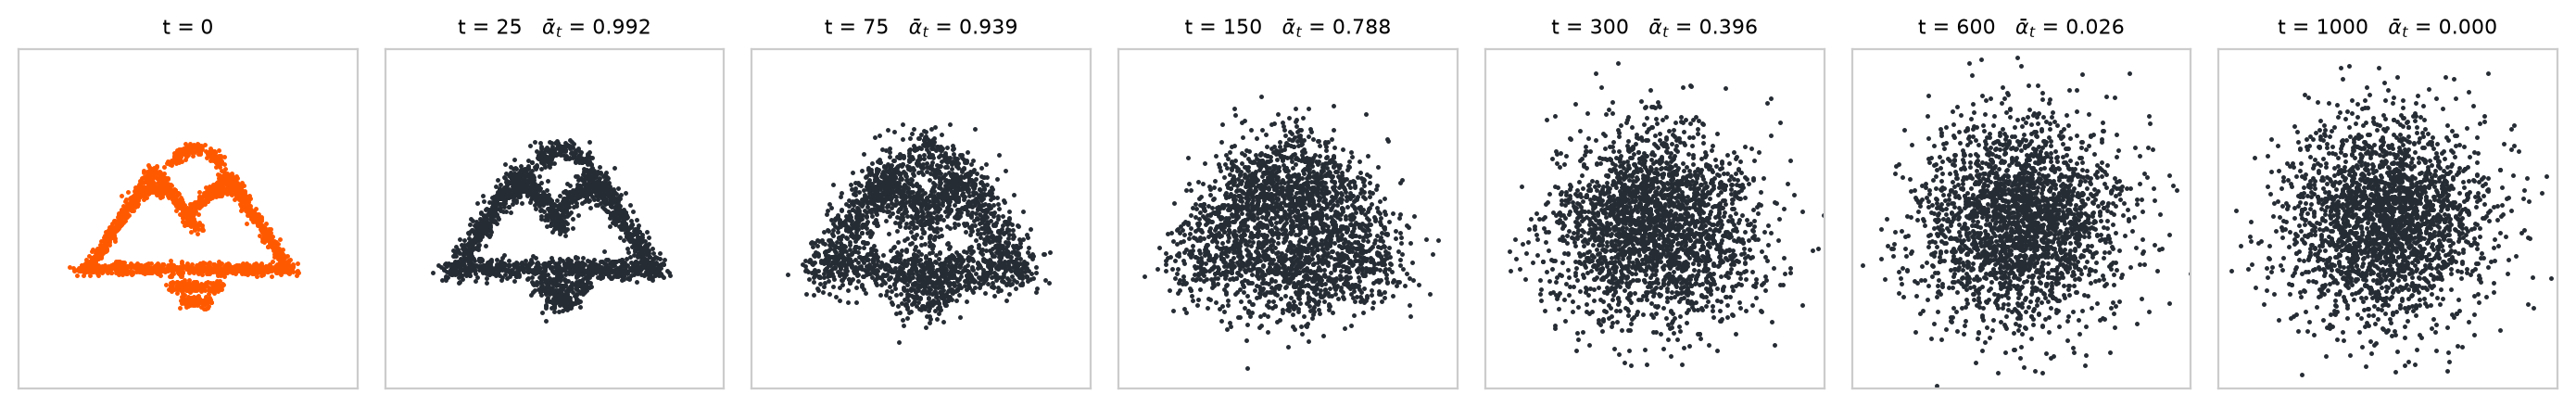
\includegraphics[width=\linewidth]{directo_2d.png}
\caption{Escalones 2 y 3 sobre datos reales. La nube de 2\,400 puntos con forma de montañas al atardecer (con su sol y sus reflejos) se disuelve en ruido gaussiano siguiendo la forma cerrada con el horario lineal. Cada panel usa el mismo $\eb$ por punto, de modo que el cambio entre paneles se debe solo a $\ab_t$.}
\label{fig:directo}
\end{figure}

\begin{ejercicio}
Despeja $\xb_0$ de la forma cerrada. Si una red pudiera adivinar $\eb$ a partir de $\xb_t$, ¿cómo recuperarías la imagen limpia? (Esta cuenta reaparece en la sección~\ref{sec:inverso}.)
\end{ejercicio}

\begin{ejercicio}
Demuestra que $\operatorname{Cov}(\xb_s,\xb_t\mid\xb_0)=\sqrt{\ab_t/\ab_s}\,(1-\ab_s)\Ib$ para $s<t$.
\end{ejercicio}

\section{Horarios de ruido: lineal y coseno}\label{sec:horarios}

El horario $\{\beta_t\}$ decide a qué velocidad se destruye la información. Dos opciones dominan la práctica.

\begin{definicion}[Horario lineal]
Ho et~al.\ (2020): $T=1000$ y $\beta_t$ crece linealmente de $\beta_1=10^{-4}$ a $\beta_T=0.02$.
\end{definicion}

\begin{definicion}[Horario coseno]
Nichol y Dhariwal (2021): se define directamente la señal acumulada
\[
\ab_t=\frac{f(t)}{f(0)},\qquad f(t)=\cos^2\!\left(\frac{t/T+s}{1+s}\cdot\frac{\pi}{2}\right),\qquad s=0.008,
\]
y se recupera $\beta_t=1-\ab_t/\ab_{t-1}$, recortado a $0.999$ para evitar singularidades cerca de $t=T$.
\end{definicion}

\begin{figure}[H]
\centering
\begin{tikzpicture}
\begin{axis}[width=0.48\linewidth, height=5.4cm, xlabel={$t$}, ylabel={$\ab_t$}, xmin=0, xmax=1000, ymin=0, ymax=1.02,
  legend style={font=\footnotesize, at={(0.97,0.97)}, anchor=north east}, grid=major, grid style={gray!20}, title={\small Señal que sobrevive}]
  \addplot[pizarra, very thick] table[x=t, y=lineal] {figuras/horarios.dat};
  \addplot[anahuac, very thick] table[x=t, y=coseno] {figuras/horarios.dat};
  \legend{lineal, coseno}
\end{axis}
\end{tikzpicture}\hfill
\begin{tikzpicture}
\begin{axis}[width=0.48\linewidth, height=5.4cm, xlabel={$t$}, ylabel={$\log_{10}\mathrm{SNR}(t)$}, xmin=0, xmax=1000,
  legend style={font=\footnotesize, at={(0.97,0.97)}, anchor=north east}, grid=major, grid style={gray!20}, title={\small Razón señal a ruido}]
  \addplot[pizarra, very thick] table[x=t, y=snrlin] {figuras/horarios.dat};
  \addplot[anahuac, very thick] table[x=t, y=snrcos] {figuras/horarios.dat};
  \legend{lineal, coseno}
\end{axis}
\end{tikzpicture}
\caption{Horarios lineal y coseno con $T=1000$, calculados con el mismo código que entrena los modelos. El lineal deja la señal por debajo de la mitad en $t=260$; el coseno, hasta $t=497$ y pasa los últimos cientos de pasos en ruido casi puro. El coseno baja con una pendiente casi constante en la zona media.}
\label{fig:horarios}
\end{figure}

La diferencia importa sobre todo en imágenes pequeñas, como las de $24\times24$ o $28\times28$ píxeles de esta sesión. Con el horario lineal, la imagen es casi irreconocible en la mitad del trayecto y los pasos finales del proceso directo aportan poco: son pasos que la red debe aprender a revertir y que casi no contienen información. El coseno reparte el trabajo de manera más pareja. Nosotros entrenamos con el horario lineal porque es el del artículo original y el que reproduce la mayoría de las implementaciones; el cuaderno y la página permiten comparar ambos.

\begin{ejercicio}
Con la aproximación $\log(1-\beta)\approx-\beta$, demuestra que el horario lineal cumple $\ab_t\approx\exp\!\big(-\beta_1t-(\beta_T-\beta_1)\tfrac{t^2}{2T}\big)$. Evalúa en $t=1000$ y compara con el valor $4.0\times10^{-5}$ que reporta el cuaderno.
\end{ejercicio}

\section{El proceso inverso: aprender a quitar ruido}\label{sec:inverso}

El escalón 4 del video dice: entrena una red neuronal para revertir esto. En pantalla aparece $f_\theta(\xb_t)\approx\xb_{t-1}$: la red recibe una imagen ruidosa y debe devolver una un poco menos ruidosa.

\subsection{El posterior que sí sabemos calcular}

Si conociéramos $q(\xb_{t-1}\mid\xb_t)$ podríamos muestrear $\xb_T\sim\Normal(\mathbf 0,\Ib)$ y recorrer la cadena al revés. Esa distribución depende de todos los datos posibles y no tiene fórmula. Pero si además conocemos el dato original $\xb_0$, el posterior sí es tratable.

\begin{teorema}[Posterior del proceso directo]\label{res:posterior}
\[
q(\xb_{t-1}\mid\xb_t,\xb_0)=\Normal\!\big(\xb_{t-1};\ \tilde{\boldsymbol\mu}_t(\xb_t,\xb_0),\ \tilde\beta_t\Ib\big),
\]
con
\[
\tilde{\boldsymbol\mu}_t(\xb_t,\xb_0)=\frac{\sqrt{\ab_{t-1}}\,\beta_t}{1-\ab_t}\,\xb_0+\frac{\sqrt{\alpha_t}\,(1-\ab_{t-1})}{1-\ab_t}\,\xb_t,
\qquad
\tilde\beta_t=\frac{1-\ab_{t-1}}{1-\ab_t}\,\beta_t .
\]
\end{teorema}

\begin{proof}
Por Bayes y la propiedad de Markov, $q(\xb_{t-1}\mid\xb_t,\xb_0)\propto q(\xb_t\mid\xb_{t-1})\,q(\xb_{t-1}\mid\xb_0)$. Ambos factores son gaussianos (el segundo por la forma cerrada), así que el logaritmo del producto es, salvo constantes que no dependen de $\xb_{t-1}$,
\[
-\frac12\left[\frac{\norm{\xb_t-\sqrt{\alpha_t}\,\xb_{t-1}}^2}{\beta_t}+\frac{\norm{\xb_{t-1}-\sqrt{\ab_{t-1}}\,\xb_0}^2}{1-\ab_{t-1}}\right].
\]
Expandimos y agrupamos por potencias de $\xb_{t-1}$. El coeficiente de $\norm{\xb_{t-1}}^2$ es
\[
\frac{\alpha_t}{\beta_t}+\frac{1}{1-\ab_{t-1}}=\frac{\alpha_t(1-\ab_{t-1})+\beta_t}{\beta_t(1-\ab_{t-1})}=\frac{1-\ab_t}{\beta_t(1-\ab_{t-1})}=\frac{1}{\tilde\beta_t},
\]
donde usamos $\alpha_t+\beta_t=1$ y $\alpha_t\ab_{t-1}=\ab_t$. El coeficiente del término lineal $-2\,\xb_{t-1}^\top(\cdot)$ es
$\frac{\sqrt{\alpha_t}}{\beta_t}\xb_t+\frac{\sqrt{\ab_{t-1}}}{1-\ab_{t-1}}\xb_0$. Completar el cuadrado da una gaussiana con varianza $\tilde\beta_t$ y media
\[
\tilde{\boldsymbol\mu}_t=\tilde\beta_t\left(\frac{\sqrt{\alpha_t}}{\beta_t}\xb_t+\frac{\sqrt{\ab_{t-1}}}{1-\ab_{t-1}}\xb_0\right)
=\frac{\sqrt{\alpha_t}(1-\ab_{t-1})}{1-\ab_t}\xb_t+\frac{\sqrt{\ab_{t-1}}\,\beta_t}{1-\ab_t}\xb_0 .\qedhere
\]
\end{proof}

La media del posterior es un promedio ponderado entre la imagen ruidosa actual y la imagen limpia. Al inicio del proceso inverso ($t$ grande) pesa más $\xb_0$; al final, pesa más $\xb_t$.

\subsection{Reescribir la media en términos del ruido}

La red no conoce $\xb_0$ cuando genera. Pero la forma cerrada permite expresarlo con el ruido: $\xb_0=\big(\xb_t-\sqrt{1-\ab_t}\,\eb\big)/\sqrt{\ab_t}$. Sustituyendo en $\tilde{\boldsymbol\mu}_t$ y simplificando (ejercicio al final de la sección):
\[
\tilde{\boldsymbol\mu}_t=\frac{1}{\sqrt{\alpha_t}}\left(\xb_t-\frac{\beta_t}{\sqrt{1-\ab_t}}\,\eb\right).
\]
Esta fórmula sugiere la parametrización de Ho et~al.\ (2020): en lugar de pedirle a la red la media, le pedimos el ruido.

\begin{definicion}[Proceso inverso parametrizado por el ruido]
Una red $\epst(\xb_t,t)$ recibe la imagen ruidosa y el paso, y estima el ruido que la contaminó. El proceso inverso es
\[
p_\theta(\xb_{t-1}\mid\xb_t)=\Normal\!\big(\xb_{t-1};\ \boldsymbol\mu_\theta(\xb_t,t),\ \sigma_t^2\Ib\big),\qquad
\boldsymbol\mu_\theta(\xb_t,t)=\frac{1}{\sqrt{\alpha_t}}\left(\xb_t-\frac{\beta_t}{\sqrt{1-\ab_t}}\,\epst(\xb_t,t)\right),
\]
con $p(\xb_T)=\Normal(\mathbf 0,\Ib)$ y varianza fija $\sigma_t^2=\tilde\beta_t$ (o $\sigma_t^2=\beta_t$; ambas funcionan casi igual).
\end{definicion}

\begin{intuicion}
El video dibuja $f_\theta(\xb_t)\approx\xb_{t-1}$. La red de un DDPM produce algo equivalente por un camino indirecto: estima qué parte de la imagen es ruido, resta una fracción pequeña de esa estimación y vuelve a agregar un poco de ruido fresco. Predecir el ruido resulta más fácil que predecir la imagen, porque el ruido siempre tiene la misma escala, sin importar $t$.
\end{intuicion}

Despejando también se obtiene la estimación de la imagen limpia en cualquier paso,
\[
\hat\xb_0(\xb_t)=\frac{\xb_t-\sqrt{1-\ab_t}\,\epst(\xb_t,t)}{\sqrt{\ab_t}},
\]
que en imágenes conviene recortar al rango válido $[-1,1]$ antes de calcular $\tilde{\boldsymbol\mu}_t(\xb_t,\hat\xb_0)$. Así lo hace nuestro script.

\begin{ejercicio}
Verifica la simplificación de $\tilde{\boldsymbol\mu}_t$: muestra que el coeficiente de $\xb_t$ es $1/\sqrt{\alpha_t}$ y el de $\eb$ es $-\beta_t/(\sqrt{\alpha_t}\sqrt{1-\ab_t})$.
\end{ejercicio}

\begin{ejercicio}
Demuestra que $\tilde\beta_t\leq\beta_t$ y que $\tilde\beta_1=0$. ¿Qué significa que la varianza del último paso inverso sea cero?
\end{ejercicio}

\section{De la verosimilitud a la pérdida simplificada}\label{sec:elbo}

Queremos elegir $\theta$ para que el modelo $p_\theta(\xb_0)=\int p_\theta(\xb_{0:T})\,d\xb_{1:T}$ asigne mucha probabilidad a los datos. La integral es intratable, pero, igual que en los autocodificadores variacionales, podemos acotarla.

\subsection{La cota inferior de la evidencia}

Para cualquier distribución $q$ sobre las variables latentes, la desigualdad de Jensen da
\[
\log p_\theta(\xb_0)=\log\E_{q(\xb_{1:T}\mid\xb_0)}\!\left[\frac{p_\theta(\xb_{0:T})}{q(\xb_{1:T}\mid\xb_0)}\right]
\geq\E_{q}\!\left[\log\frac{p_\theta(\xb_{0:T})}{q(\xb_{1:T}\mid\xb_0)}\right]\eqqcolon\mathrm{ELBO}.
\]
La gracia de la difusión es que el ``codificador'' $q$ está fijo: es el proceso directo, sin parámetros. Solo se aprende el decodificador $p_\theta$.

\begin{teorema}[Descomposición de la ELBO]\label{res:elbo}
Usando $q(\xb_t\mid\xb_{t-1})=q(\xb_t\mid\xb_{t-1},\xb_0)$ y la regla de Bayes para reescribir cada factor como $q(\xb_{t-1}\mid\xb_t,\xb_0)\,q(\xb_t\mid\xb_0)/q(\xb_{t-1}\mid\xb_0)$, la ELBO negativa se descompone como
\begin{multline*}
-\mathrm{ELBO}=\underbrace{\KL\!\big(q(\xb_T\mid\xb_0)\,\Vert\,p(\xb_T)\big)}_{L_T}
+\sum_{t=2}^{T}\underbrace{\E_q\,\KL\!\big(q(\xb_{t-1}\mid\xb_t,\xb_0)\,\Vert\,p_\theta(\xb_{t-1}\mid\xb_t)\big)}_{L_{t-1}}\\
\underbrace{-\,\E_q\log p_\theta(\xb_0\mid\xb_1)}_{L_0}.
\end{multline*}
\end{teorema}

Cada término tiene una lectura sencilla:
\begin{itemize}
  \item $L_T$ mide si el proceso directo termina realmente en ruido estándar. No tiene parámetros y, con $\ab_T\approx4\times10^{-5}$, vale prácticamente cero.
  \item $L_{t-1}$ compara el paso inverso aprendido con el posterior verdadero, que sí conocemos gracias al resultado~\ref{res:posterior}. Es una KL entre dos gaussianas.
  \item $L_0$ es un término de reconstrucción del último paso.
\end{itemize}

\subsection{Cada término es una regresión}

Como $q(\xb_{t-1}\mid\xb_t,\xb_0)$ y $p_\theta(\xb_{t-1}\mid\xb_t)$ son gaussianas con varianzas fijas, el resultado~\ref{res:kl} da (tomando $\sigma_t^2$ como la varianza común)
\[
L_{t-1}=\E_q\left[\frac{1}{2\sigma_t^2}\norm{\tilde{\boldsymbol\mu}_t(\xb_t,\xb_0)-\boldsymbol\mu_\theta(\xb_t,t)}^2\right]+C .
\]
Sustituimos las dos medias escritas con el ruido. El término $\xb_t/\sqrt{\alpha_t}$ se cancela y queda
\[
L_{t-1}=\E_{\xb_0,\eb}\left[\frac{\beta_t^2}{2\sigma_t^2\,\alpha_t\,(1-\ab_t)}\,\norm{\eb-\epst\big(\sqrt{\ab_t}\,\xb_0+\sqrt{1-\ab_t}\,\eb,\ t\big)}^2\right]+C .
\]
Toda la maquinaria probabilística se redujo a esto: \textbf{adivinar el ruido}, con un peso que depende de $t$.

\begin{definicion}[Pérdida simplificada]
Ho et~al.\ (2020) descartan los pesos y sortean $t$ de manera uniforme:
\[
L_{\text{simple}}(\theta)=\E_{t\sim\mathcal U\{1,\dots,T\},\ \xb_0\sim q,\ \eb\sim\Normal(\mathbf 0,\Ib)}
\Big[\norm{\eb-\epst\big(\sqrt{\ab_t}\,\xb_0+\sqrt{1-\ab_t}\,\eb,\ t\big)}^2\Big].
\]
\end{definicion}

\begin{intuicion}
Descartar los pesos parece un descuido y resulta una mejora. Los pesos originales son enormes para $t$ pequeño, donde el ruido es casi imperceptible y la tarea es fácil. Quitarlos le da más importancia relativa a los niveles de ruido intermedios y altos, donde la red tiene que ``imaginar'' estructura, y eso produce muestras de mejor calidad visual. El precio es que $L_{\text{simple}}$ ya no es exactamente una cota de la verosimilitud.
\end{intuicion}

\begin{figure}[H]
\centering
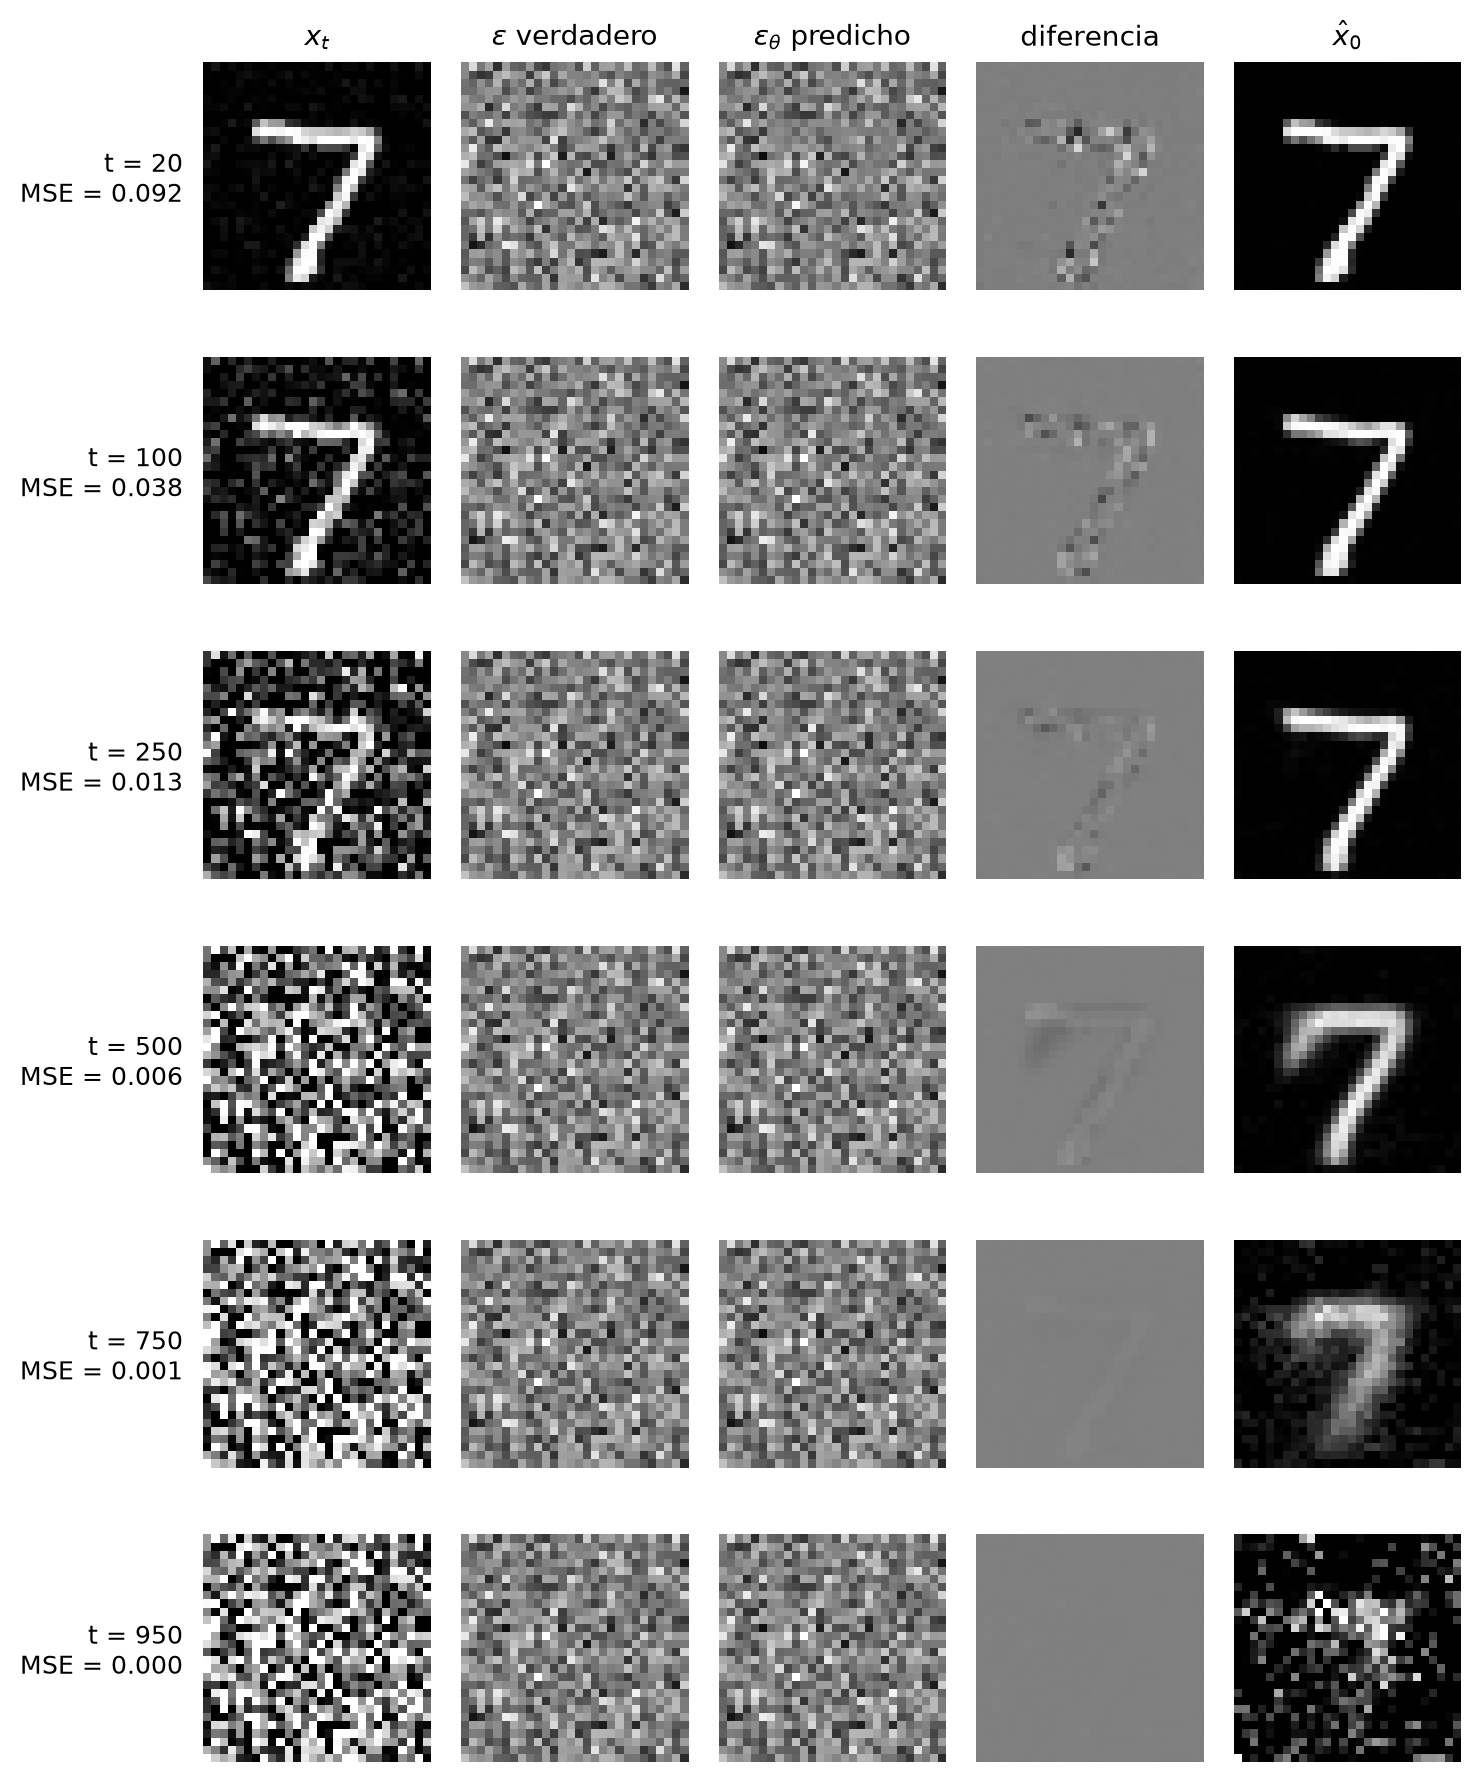
\includegraphics[width=0.92\linewidth]{perdida_detalle.png}
\caption{La pérdida vista por dentro, con la U-Net entrenada sobre MNIST. Para un dígito de prueba se fabrica $\xb_t$ con un ruido conocido. La red predice el ruido; la diferencia con el verdadero es lo que penaliza $L_{\text{simple}}$. La última columna despeja $\hat\xb_0$. Con $t$ pequeño, el error se concentra en los bordes del trazo; con $t$ grande, la red ya ``ve'' un 7 en medio del ruido.}
\label{fig:perdida-detalle}
\end{figure}

\begin{figure}[H]
\centering
\begin{tikzpicture}
\begin{axis}[width=0.62\linewidth, height=5cm, xlabel={$t$}, ylabel={MSE del ruido}, xmin=0, xmax=1000, ymin=0,
  legend style={font=\footnotesize, at={(0.97,0.97)}, anchor=north east}, grid=major, grid style={gray!20}]
  \addplot[anahuac, very thick] table[x=t, y=mnist] {figuras/perdida_t.dat};
  \addplot[pizarra, very thick] table[x=t, y=montanas] {figuras/perdida_t.dat};
  \legend{MNIST (U-Net), montañas 2D (MLP)}
\end{axis}
\end{tikzpicture}
\caption{Error de predicción del ruido según el nivel de ruido, medido con los modelos entrenados. En 2D el error es alto para $t$ pequeño: un punto apenas desplazado de la forma no revela hacia dónde se movió a lo largo de ella. En imágenes ocurre lo contrario cerca de $t=T$, donde la red debe inventar casi todo.}
\label{fig:perdida-t}
\end{figure}

\begin{ejercicio}
Calcula el peso $\lambda_t=\beta_t^2/(2\sigma_t^2\alpha_t(1-\ab_t))$ con $\sigma_t^2=\beta_t$ para $t=1$, $t=100$ y $t=1000$ con el horario lineal. ¿Cuántos órdenes de magnitud separan el primero del último?
\end{ejercicio}

\begin{ejercicio}
Muestra que, si la red predice $\hat\xb_0$ en lugar de $\eb$, la pérdida equivalente es $\norm{\xb_0-\hat\xb_0}^2$ multiplicada por $\mathrm{SNR}(t)$ (salvo constantes). ¿Qué nivel de ruido domina entonces?
\end{ejercicio}

\section{Los algoritmos de entrenamiento y muestreo}\label{sec:algoritmos}

El escalón 6 del video dice: entrena el modelo con imágenes en todos los niveles de ruido. Es exactamente lo que hace el paso 2 del algoritmo de entrenamiento al sortear $t$.

\begin{algoritmo}{Algoritmo 1. Entrenamiento (DDPM)}
  \item \textbf{repetir}
  \item \quad $\xb_0\sim q(\xb_0)$ \hfill (un dato del conjunto de entrenamiento)
  \item \quad $t\sim\mathcal U\{1,\dots,T\}$ \hfill (un nivel de ruido al azar)
  \item \quad $\eb\sim\Normal(\mathbf 0,\Ib)$
  \item \quad $\xb_t\leftarrow\sqrt{\ab_t}\,\xb_0+\sqrt{1-\ab_t}\,\eb$ \hfill (forma cerrada, un solo salto)
  \item \quad dar un paso de gradiente sobre $\nabla_\theta\norm{\eb-\epst(\xb_t,t)}^2$
  \item \textbf{hasta} converger
\end{algoritmo}

\begin{algoritmo}{Algoritmo 2. Muestreo (rebobinar el video)}
  \item $\xb_T\sim\Normal(\mathbf 0,\Ib)$
  \item \textbf{para} $t=T,\dots,1$ \textbf{hacer}
  \item \quad $\zb\sim\Normal(\mathbf 0,\Ib)$ si $t>1$; si no, $\zb=\mathbf 0$
  \item \quad $\xb_{t-1}\leftarrow\dfrac{1}{\sqrt{\alpha_t}}\left(\xb_t-\dfrac{\beta_t}{\sqrt{1-\ab_t}}\,\epst(\xb_t,t)\right)+\sigma_t\zb$
  \item \textbf{devolver} $\xb_0$
\end{algoritmo}

El entrenamiento es barato: cada iteración usa una sola evaluación de la red. El muestreo es caro: requiere $T$ evaluaciones en secuencia. Esta asimetría motivó una familia entera de muestreadores acelerados, como DDIM (Song, Meng y Ermon, 2021), que reinterpreta el mismo modelo entrenado como un proceso determinista y genera con 50 pasos o menos.

\begin{lstlisting}[language=Python, caption={El corazón de \texttt{scripts/train\_ddpm.py}: una iteración de entrenamiento y un paso de muestreo.}]
# Entrenamiento: algoritmo 1
t = torch.randint(0, T, (len(x0),), device=DEVICE)    # índice 0..T-1
eps = torch.randn_like(x0)
x_t = ab[t].sqrt() * x0 + (1 - ab[t]).sqrt() * eps    # forma cerrada
perdida = F.mse_loss(modelo(x_t, t), eps)

# Muestreo: un paso del algoritmo 2
media = (x - betas[i] / (1 - ab[i]).sqrt() * eps_pred) / alphas[i].sqrt()
x = media + var_post[i].sqrt() * torch.randn_like(x)   # sigma_t^2 = beta tilde
\end{lstlisting}

\begin{nota}[Los modelos de esta sesión]
Los cuatro modelos usan $T=1000$, horario lineal, AdamW y semilla 42. Los modelos 2D son un MLP residual de cuatro capas de ancho 256 con codificación sinusoidal de $t$, entrenado 16\,000 pasos con lotes de 2\,048 puntos. Los modelos de imágenes son una U-Net de 2.9 millones de parámetros (tres resoluciones, bloques residuales con normalización por grupos y una capa de autoatención en la resolución más baja), con promedio exponencial de pesos para muestrear. El cuadro~\ref{tab:metricas} resume las corridas.
\end{nota}

% Generado por scripts/figuras_difusion.py
\begin{table}[H]
\centering\small
\begin{tabular}{lllrrr}
\toprule
Modelo & Red & Datos & Entrenamiento & $L_{\text{simple}}$ final & Tiempo (s)\\
\midrule
Montañas 2D & MLP & 60\,000 puntos & 16\,000 pasos & 0.2292 & 73\\
Letras UA 2D & MLP & 60\,000 puntos & 16\,000 pasos & 0.2208 & 73\\
Paisajes $24\times24$ & U-Net condicional & 36\,000 imágenes & 14 épocas & 0.0202 & 252\\
MNIST $28\times28$ & U-Net condicional & 60\,000 imágenes & 12 épocas & 0.0225 & 488\\
\bottomrule
\end{tabular}
\caption{Corridas de \texttt{scripts/train\_ddpm.py} en una NVIDIA GeForce RTX 3070 Laptop GPU. Tiempo total con muestreo y exportación: 15.8 minutos; pico de memoria de GPU: 735 MB.}
\label{tab:metricas}
\end{table}


\begin{figure}[H]
\centering
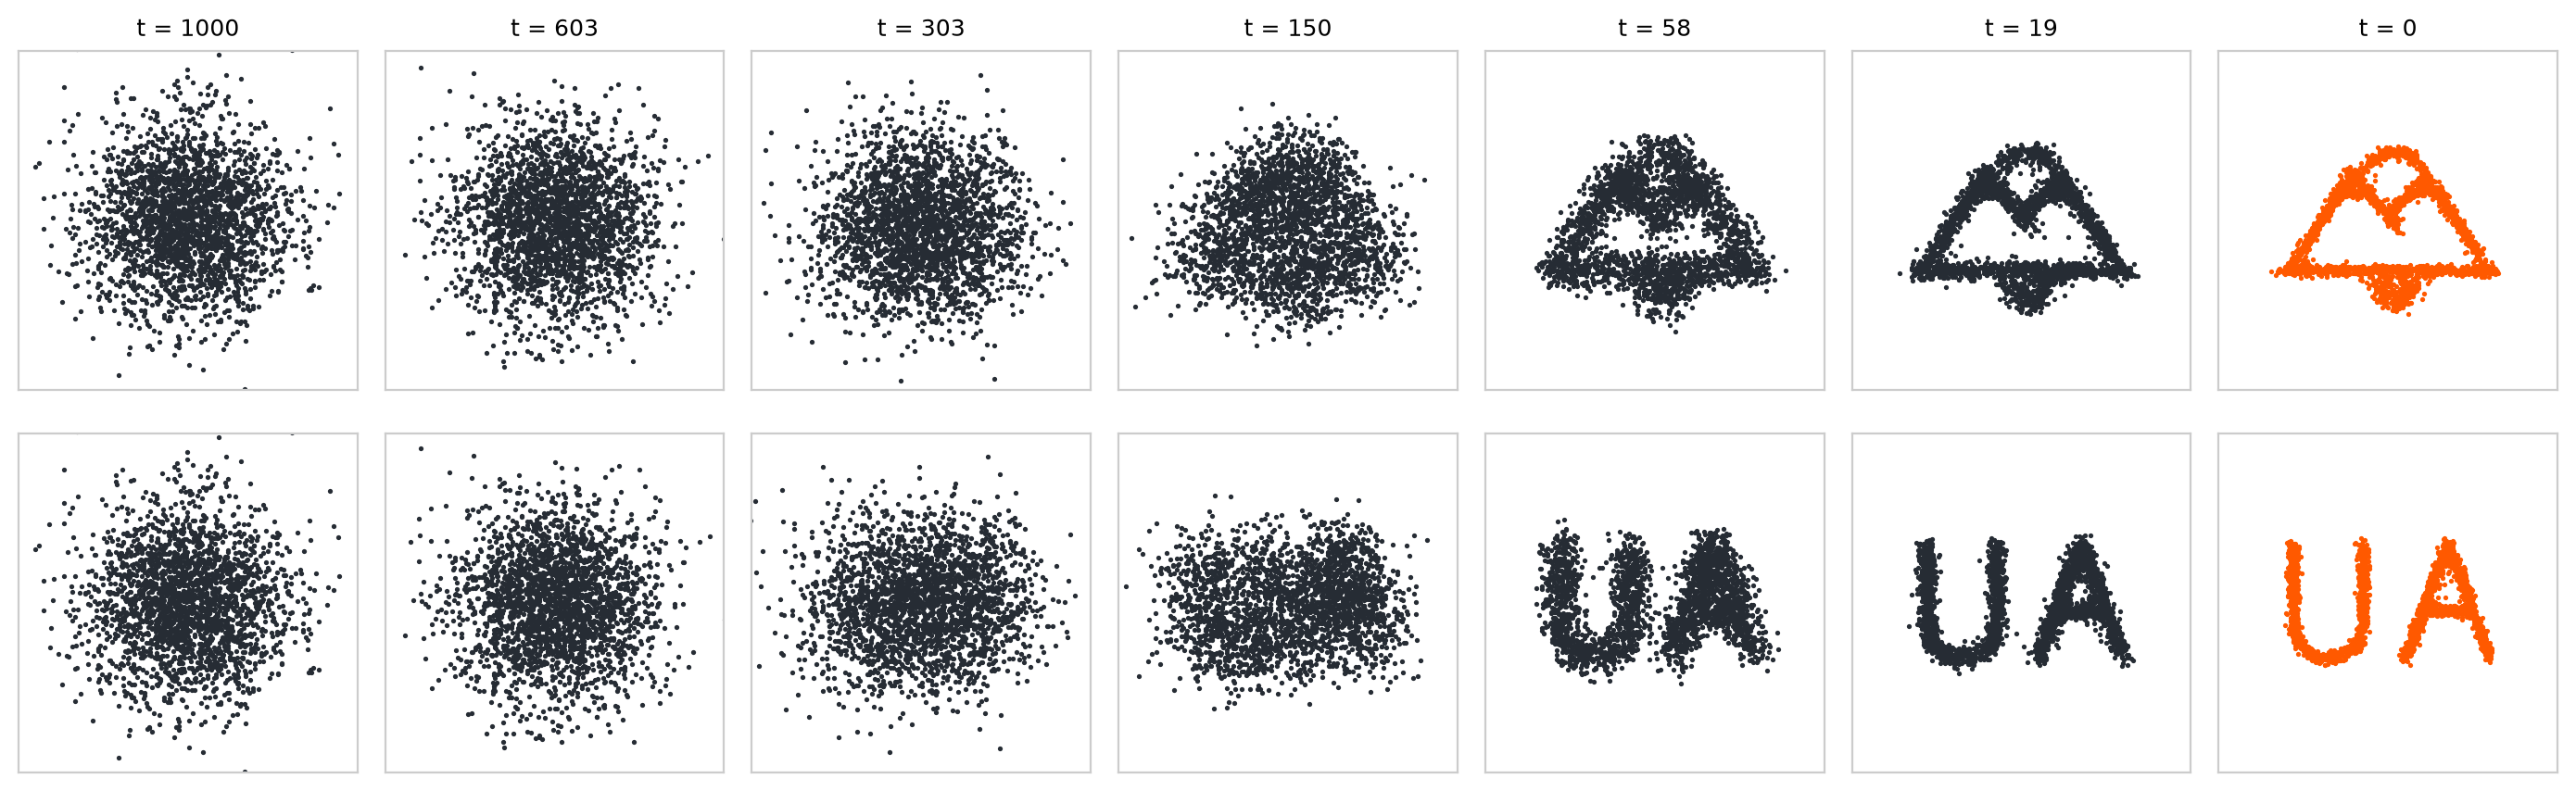
\includegraphics[width=\linewidth]{inverso_2d.png}
\caption{Algoritmo 2 sobre los modelos 2D: 1\,200 partículas parten de ruido puro ($t=1000$) y, guiadas por la red, se reensamblan en las montañas (arriba) y en las letras UA (abajo). Las trayectorias completas alimentan la animación de la página interactiva.}
\label{fig:inverso}
\end{figure}

\begin{ejercicio}
¿Cuántas evaluaciones de la red cuesta generar 16 dígitos con $T=1000$ y guía sin clasificador? (Pista: la guía necesita dos evaluaciones por paso.)
\end{ejercicio}

\begin{ejercicio}
En el algoritmo 1, ¿qué pasaría si $t$ se sorteara siempre igual a 1? ¿Y si se sorteara siempre igual a $T$? Relaciona tu respuesta con la figura~\ref{fig:perdida-t}.
\end{ejercicio}

\section{El score y la dinámica de Langevin}\label{sec:score}

Hay otra manera de mirar la red de ruido, que conecta la difusión con una tradición más antigua de la física estadística.

\begin{definicion}[Score]
El \emph{score} de una densidad $p(\xb)$ es el gradiente de su logaritmo, $\nabla_\xb\log p(\xb)$. Es un campo vectorial que en cada punto señala la dirección en la que la densidad crece más rápido.
\end{definicion}

El score no requiere conocer la constante de normalización de $p$, porque $\nabla\log(p/Z)=\nabla\log p$. Si conocemos el score, podemos muestrear de $p$ con la \emph{dinámica de Langevin}:
\[
\xb_{k+1}=\xb_k+\frac{\eta}{2}\,\nabla_\xb\log p(\xb_k)+\sqrt{\eta}\,\zb_k,\qquad \zb_k\sim\Normal(\mathbf 0,\Ib).
\]
El primer término empuja cuesta arriba en la densidad; el segundo agrega agitación para no quedarse en un solo máximo. Con $\eta\to0$ y muchas iteraciones, la cadena produce muestras de $p$.

\begin{teorema}[La red de ruido estima el score]\label{res:score}
Para la distribución ruidosa $q_t(\xb_t)=\int q(\xb_t\mid\xb_0)\,q(\xb_0)\,d\xb_0$,
\[
\nabla_{\xb_t}\log q_t(\xb_t)=-\frac{\E\big[\eb\mid\xb_t\big]}{\sqrt{1-\ab_t}},
\qquad\text{y por lo tanto}\qquad
s_\theta(\xb_t,t)\coloneqq-\frac{\epst(\xb_t,t)}{\sqrt{1-\ab_t}}\approx\nabla_{\xb_t}\log q_t(\xb_t).
\]
\end{teorema}

\begin{proof}[Idea de la demostración]
Para un $\xb_0$ fijo, $\nabla_{\xb_t}\log q(\xb_t\mid\xb_0)=-(\xb_t-\sqrt{\ab_t}\,\xb_0)/(1-\ab_t)=-\eb/\sqrt{1-\ab_t}$. El score de la mezcla es el promedio de estos gradientes condicionales con pesos $q(\xb_0\mid\xb_t)$, es decir, $-\E[\eb\mid\xb_t]/\sqrt{1-\ab_t}$. Por otro lado, el minimizador de $\E\norm{\eb-\epst(\xb_t,t)}^2$ es justamente la esperanza condicional $\E[\eb\mid\xb_t]$. Este argumento se conoce como \emph{denoising score matching} (Vincent, 2011) y también como fórmula de Tweedie.
\end{proof}

Leído así, el paso de muestreo del algoritmo 2 es un paso de Langevin con temperatura y tamaño de paso que cambian con $t$:
\[
\xb_{t-1}=\frac{1}{\sqrt{\alpha_t}}\Big(\xb_t+\beta_t\,s_\theta(\xb_t,t)\Big)+\sigma_t\zb .
\]
Song et~al.\ (2021) mostraron que, cuando $T\to\infty$, el proceso directo es una ecuación diferencial estocástica y el inverso es otra cuyo término de deriva es el score. DDPM y los modelos basados en score son dos caras de la misma idea.

\begin{figure}[H]
\centering
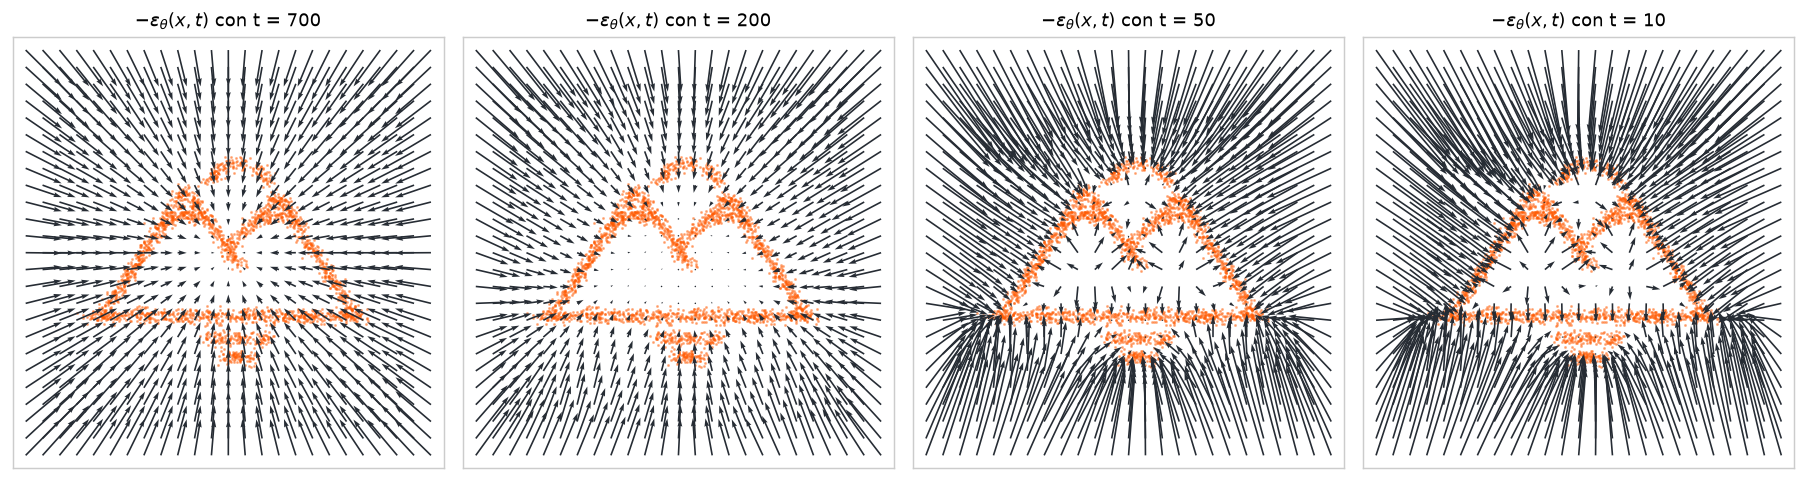
\includegraphics[width=\linewidth]{score_2d.png}
\caption{El campo $-\epst(\xb,t)$ del modelo de montañas en cuatro niveles de ruido, sobre los datos en naranja. Con $t$ grande, las flechas apuntan casi radialmente hacia el centro de masa de la nube. Al bajar $t$, el campo se pliega sobre la forma: las flechas señalan hacia la montaña o el sol más cercano.}
\label{fig:score}
\end{figure}

\begin{intuicion}
Imagina el plano como un terreno cuya altura es $\log q_t$. Con mucho ruido el terreno es una colina suave con una sola cima en el centro. Al reducir el ruido aparecen crestas con la forma de las montañas. Las partículas del proceso inverso son canicas que ruedan cuesta arriba mientras alguien sacude el terreno cada vez con menos fuerza.
\end{intuicion}

\begin{ejercicio}
Calcula el score de $\Normal(\boldsymbol\mu,\sigma^2\Ib)$. Escribe la dinámica de Langevin para esa distribución y verifica que su distribución estacionaria es la propia gaussiana cuando $\eta\to0$.
\end{ejercicio}

\begin{ejercicio}
Sustituye $s_\theta=-\epst/\sqrt{1-\ab_t}$ en la expresión de Langevin de esta sección y comprueba que coincide con el paso del algoritmo 2.
\end{ejercicio}

\section{Condicionar: decirle a la red qué quieres ver}\label{sec:guia}

El escalón 5 del video agrega una entrada: el texto ``mountains at sunset'' entra a la red junto con la imagen ruidosa, y la red pasa a ser $f_\theta(\xb_t,t,c)$. Si con la misma imagen ruidosa escribimos ``a city at night'', el resultado cambia.

\subsection{Modelos condicionales}

La extensión directa es entrenar $\epst(\xb_t,t,c)$ con pares $(\xb_0,c)$, donde $c$ es una etiqueta o la representación de un texto. En nuestra U-Net, $c$ entra como un vector aprendido que se suma a la codificación de $t$ en cada bloque residual. En Stable Diffusion, el texto entra por atención cruzada.

En la práctica, el modelo condicional por sí solo suele ignorar parcialmente la condición. Necesitamos una perilla que regule cuánto caso le hace.

\subsection{Guía sin clasificador}

Por la regla de Bayes, $\log p(\xb\mid c)=\log p(\xb)+\log p(c\mid\xb)-\log p(c)$, y en términos de scores
\[
\nabla_\xb\log p(\xb\mid c)=\nabla_\xb\log p(\xb)+\nabla_\xb\log p(c\mid\xb).
\]
El segundo término es el gradiente de un clasificador: empuja la muestra hacia donde el clasificador está seguro de que es de clase $c$. Dhariwal y Nichol (2021) lo amplificaron con un factor $w$ usando un clasificador entrenado sobre imágenes ruidosas. Ho y Salimans (2022) observaron que el clasificador sobra, porque el mismo gradiente se obtiene restando dos scores: $\nabla\log p(c\mid\xb)=\nabla\log p(\xb\mid c)-\nabla\log p(\xb)$.

\begin{definicion}[Guía sin clasificador]
Se entrena una sola red que a veces recibe la condición $c$ y a veces una condición nula $\varnothing$ (en nuestro caso, el 15 \% de las veces). Al muestrear se combinan las dos predicciones:
\[
\tilde\eb_\theta(\xb_t,t,c)=\epst(\xb_t,t,\varnothing)+w\,\big(\epst(\xb_t,t,c)-\epst(\xb_t,t,\varnothing)\big).
\]
Con $w=0$ el modelo ignora la condición; con $w=1$ es el modelo condicional; con $w>1$ exagera lo que distingue a $c$ de todo lo demás.
\end{definicion}

\begin{nota}[Dos convenciones]
Ho y Salimans (2022) escriben $(1+w)\,\epst(\cdot,c)-w\,\epst(\cdot,\varnothing)$, de modo que su $w=0$ es el modelo condicional. Aquí usamos la convención de Stable Diffusion (``guidance scale''), donde el modelo condicional corresponde a $w=1$ y los valores habituales están entre 5 y 9.
\end{nota}

\begin{figure}[H]
\centering
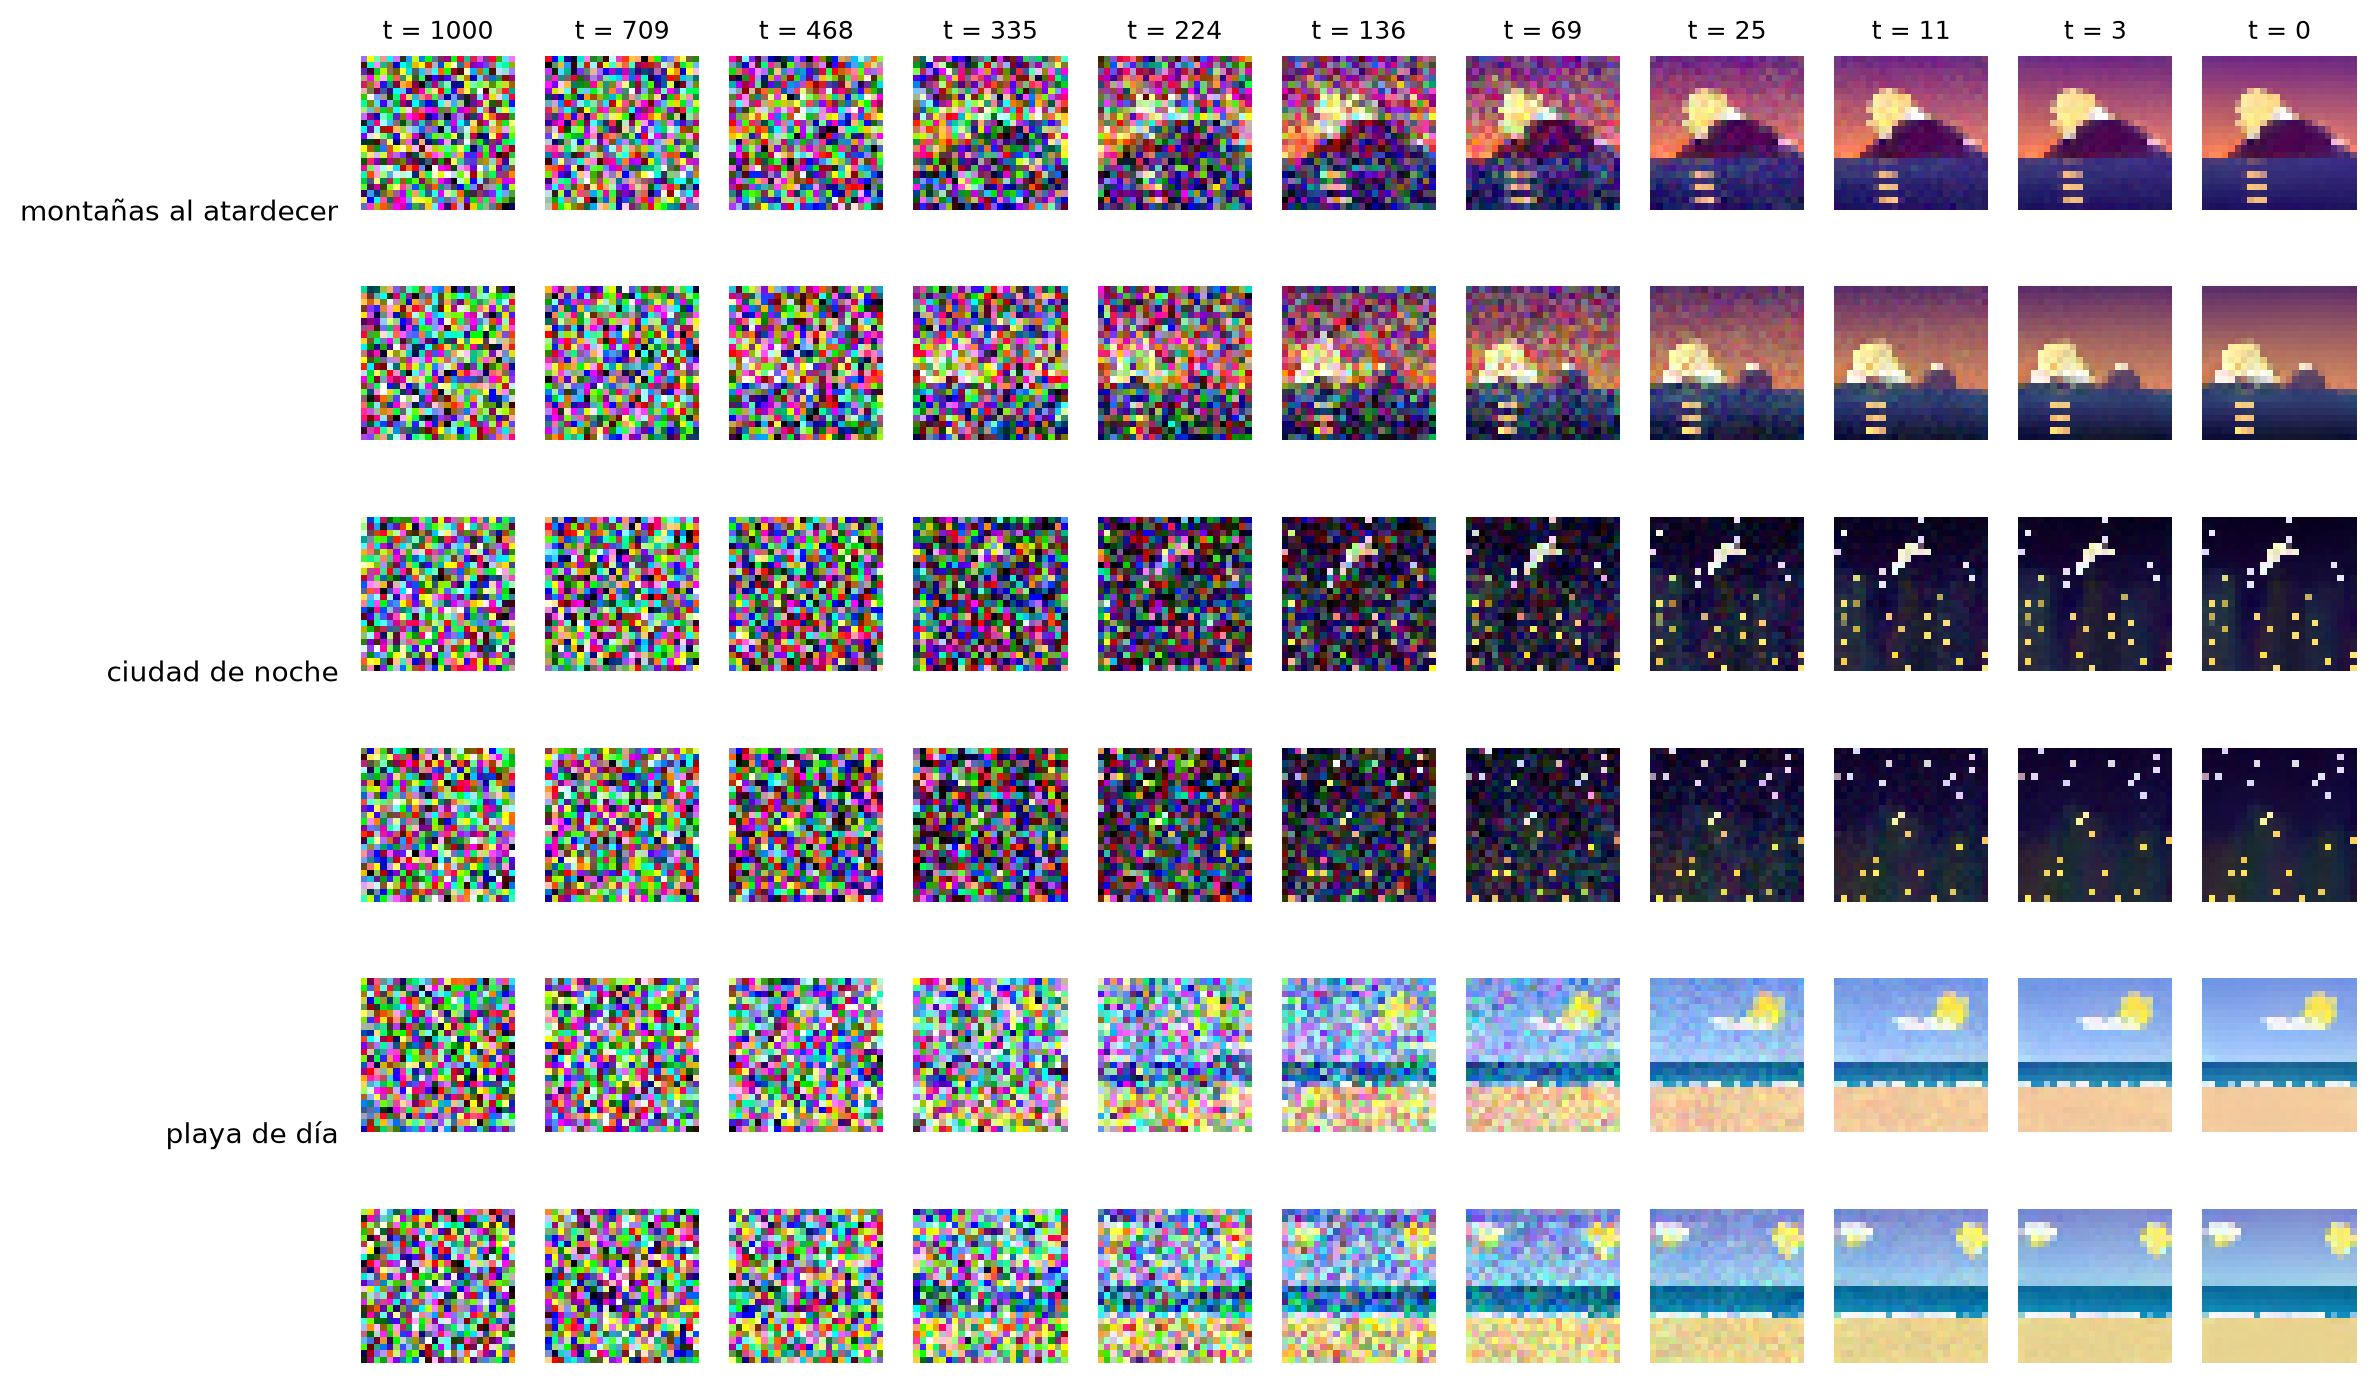
\includegraphics[width=\linewidth]{paisajes_tira.png}
\caption{Escalones 5 y 6 con un modelo real. Una U-Net condicional entrenada con 36\,000 paisajes de pixel art de $24\times24$ recorre $t=T\ldots1$ con guía $w=3$ para tres ``prompts''. Es el bucle del video, $f_\theta(\xb_t,t,c)$, con nuestras propias montañas al atardecer.}
\label{fig:paisajes}
\end{figure}

\begin{figure}[H]
\centering
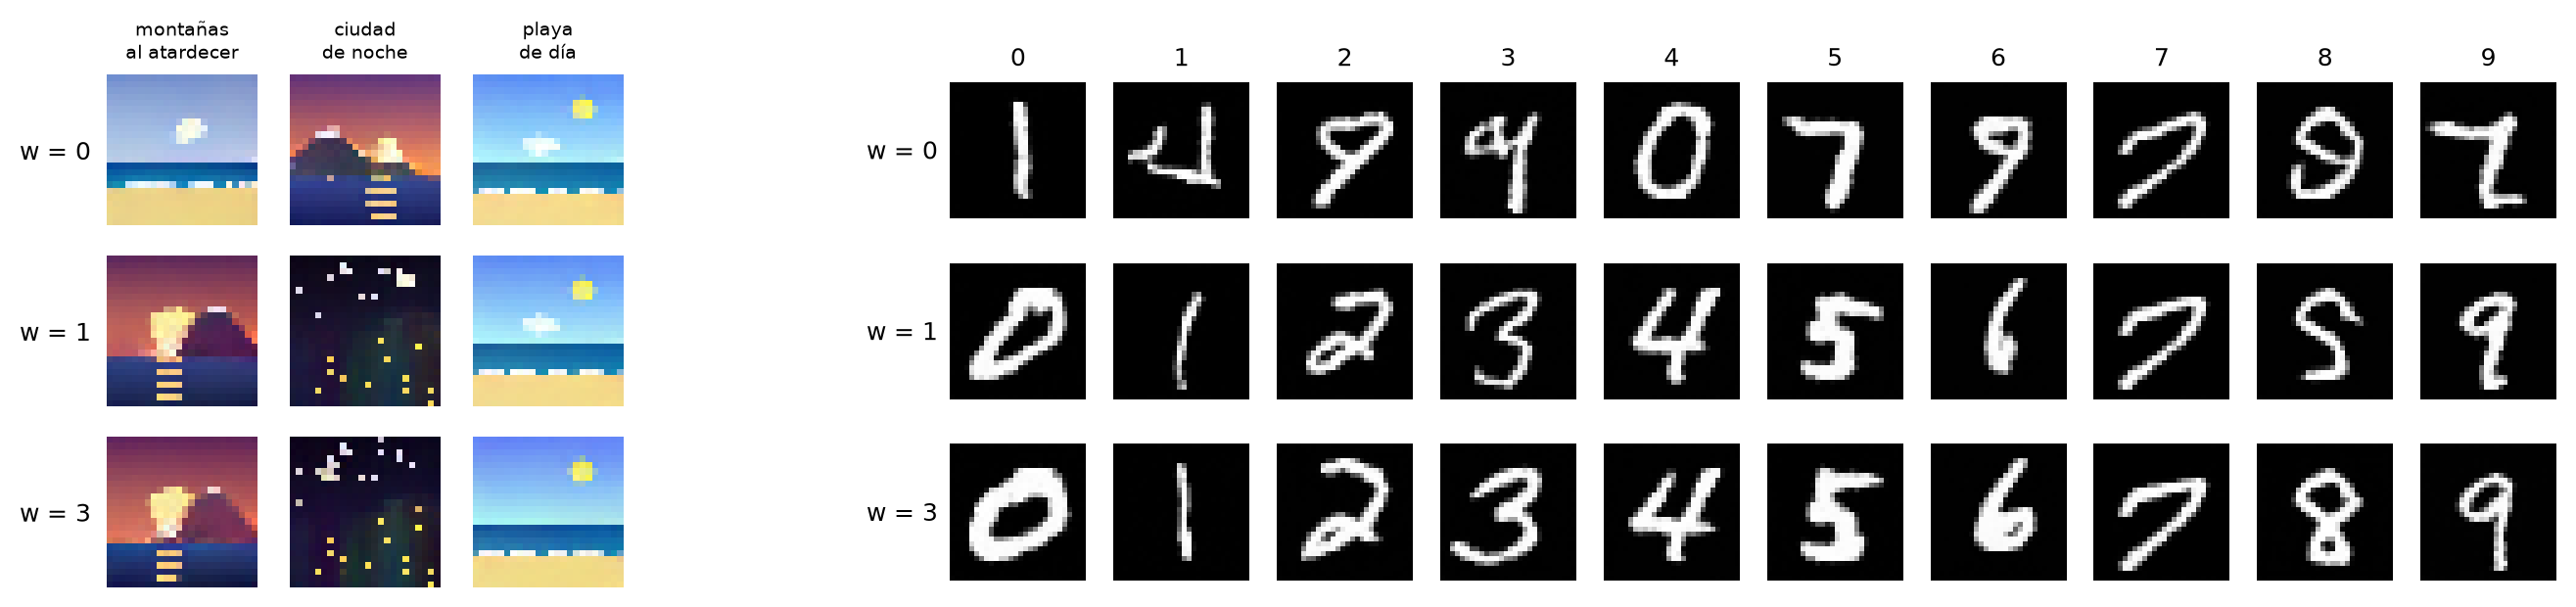
\includegraphics[width=0.95\linewidth]{guia.png}
\caption{Efecto de la escala de guía con el \emph{mismo} ruido inicial. Izquierda: paisajes (filas: $w=0,1,3$; columnas: los tres prompts). Derecha: dígitos de MNIST (columnas: clases 0 a 9). Con $w=0$ la clase es arbitraria; con $w=3$ la imagen obedece al prompt y gana contraste a costa de diversidad.}
\label{fig:guia}
\end{figure}

\begin{figure}[H]
\centering
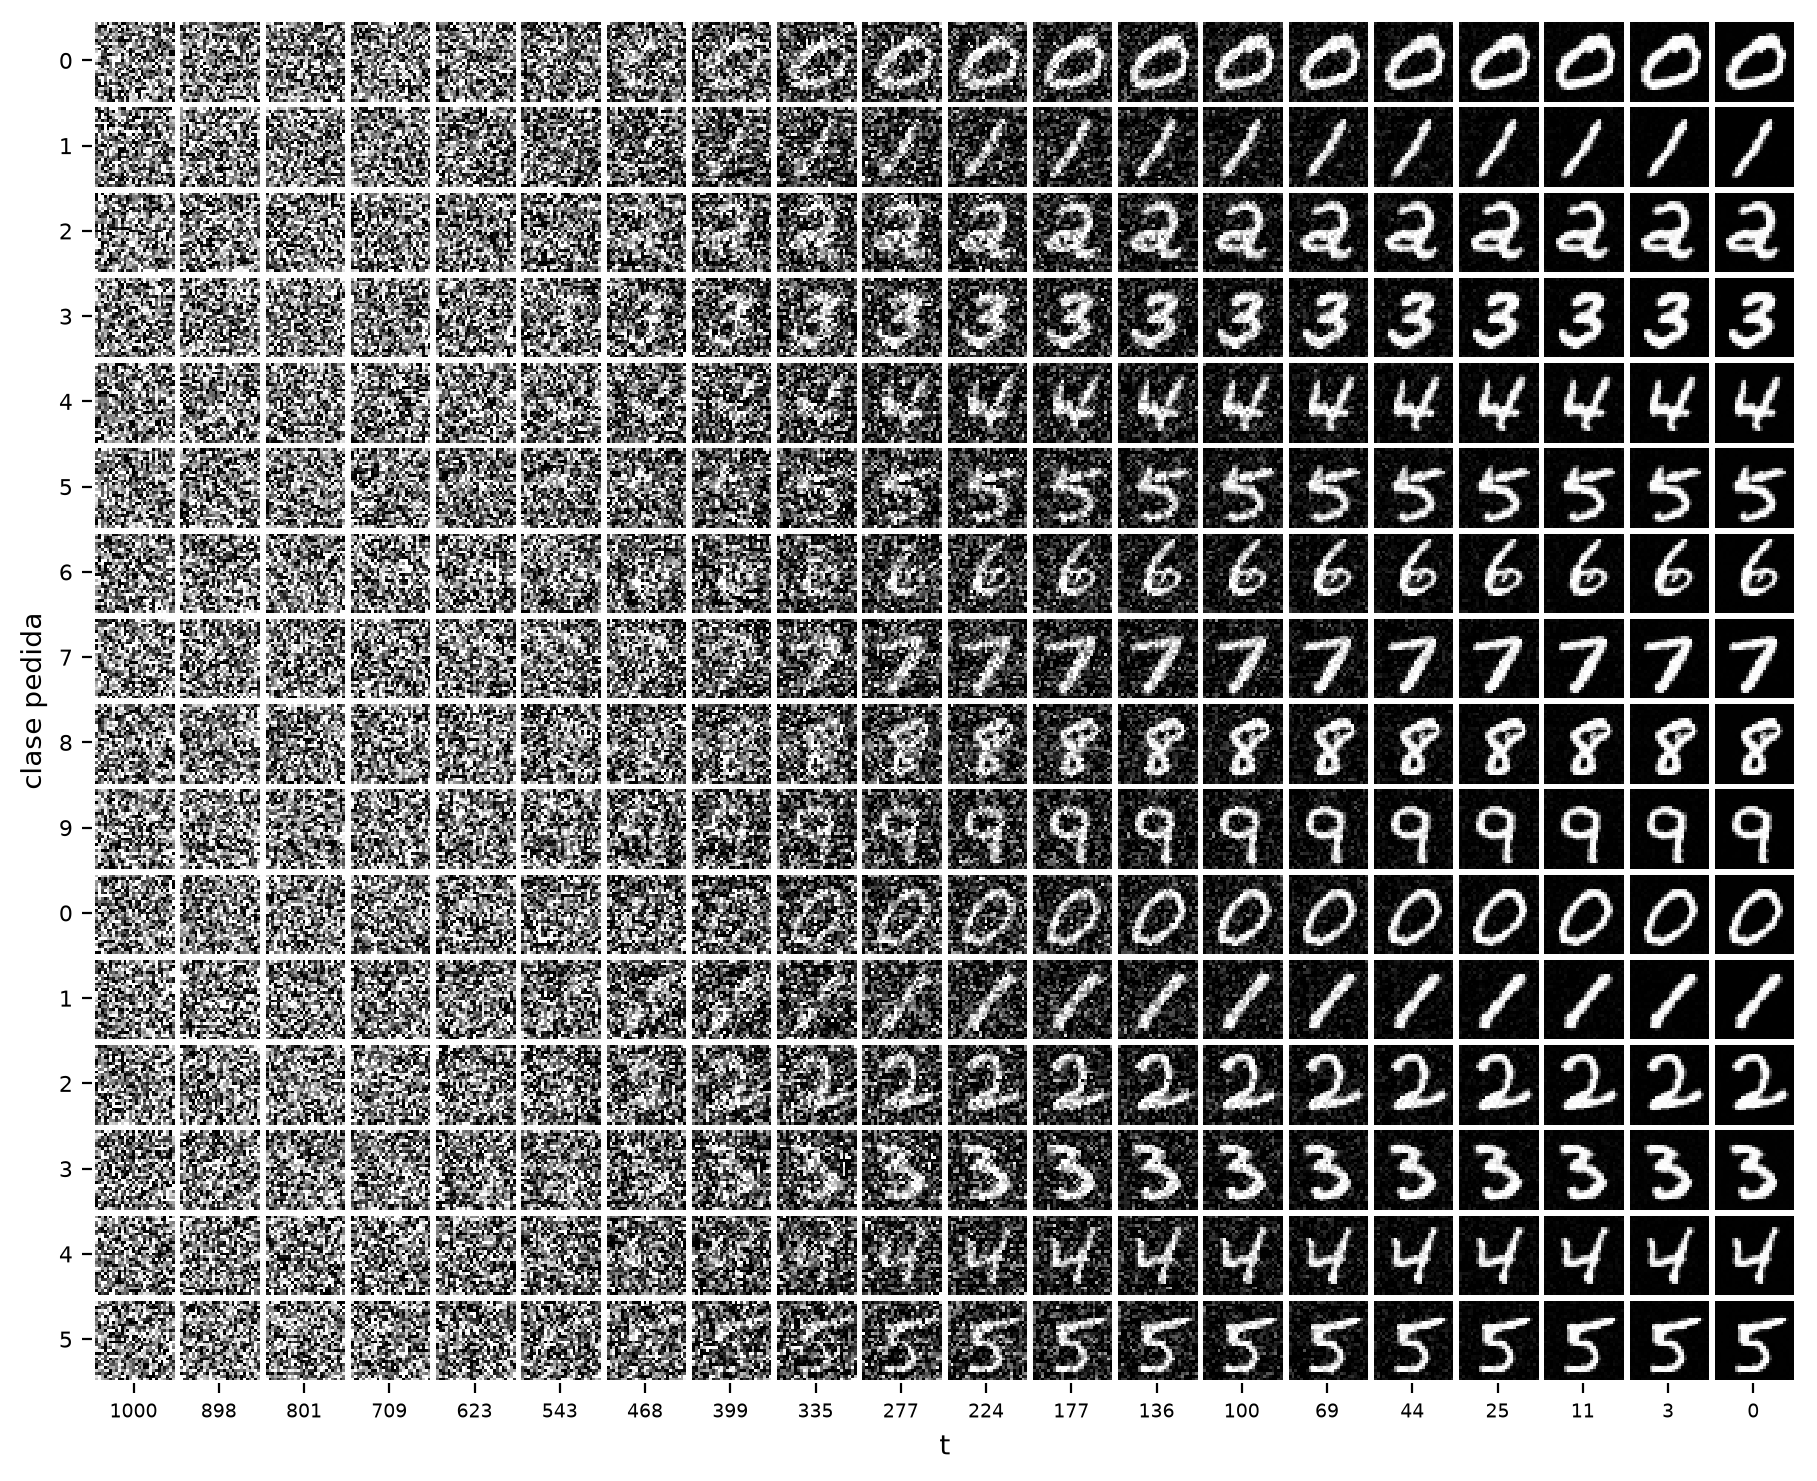
\includegraphics[width=0.9\linewidth]{mnist_tira.png}
\caption{Dieciséis dígitos naciendo del ruido con la U-Net condicional de MNIST y guía $w=2$. Cada fila es una trayectoria del algoritmo 2 en 20 instantes, más densos al final, donde aparecen los detalles.}
\label{fig:mnist}
\end{figure}

\begin{ejercicio}
Muestra que la guía sin clasificador equivale a muestrear de una distribución proporcional a $p(\xb)\,p(c\mid\xb)^w$. ¿Por qué un $w$ grande reduce la diversidad?
\end{ejercicio}

\begin{ejercicio}
Con la guía, ¿cuántas evaluaciones de red cuesta cada paso? Propón una forma de reducir ese costo a una sola pasada (pista: el lote).
\end{ejercicio}

\section{Difusión latente: el escalón de los millones de imágenes}\label{sec:latente}

El escalón 7 del video salta a escala industrial: millones de imágenes con sus descripciones. Hacer difusión directamente sobre imágenes de $512\times512\times3$ (786\,432 números) es carísimo, porque cada uno de los cientos de pasos de muestreo evalúa una U-Net sobre esa resolución.

\begin{definicion}[Difusión latente]
Rombach et~al.\ (2022) separan el problema en dos partes:
\begin{enumerate}
  \item Un autocodificador $(\mathcal E,\mathcal D)$, entrenado una sola vez, comprime la imagen a un \emph{latente} $\zb=\mathcal E(\xb)$ de $64\times64\times4$ (16\,384 números, 48 veces menos) y la reconstruye con $\mathcal D(\zb)\approx\xb$. Se entrena con pérdidas perceptuales y adversarias para que la reconstrucción conserve los detalles que importan al ojo.
  \item Un modelo de difusión trabaja \emph{en el espacio latente}: $\zb_t=\sqrt{\ab_t}\,\zb_0+\sqrt{1-\ab_t}\,\eb$, con pérdida $\norm{\eb-\epst(\zb_t,t,\tau(c))}^2$, donde $\tau$ es un codificador de texto (CLIP en Stable Diffusion 1.x) cuyas representaciones entran a la U-Net por atención cruzada.
\end{enumerate}
Para generar se muestrea $\zb_T\sim\Normal(\mathbf 0,\Ib)$, se aplica el algoritmo 2 con guía y se decodifica $\xb=\mathcal D(\zb_0)$.
\end{definicion}

\begin{figure}[H]
\centering
\begin{tikzpicture}[font=\sffamily\small, >={Stealth[length=2.2mm]},
  caja/.style={draw=pizarra, rounded corners=2pt, minimum height=0.9cm, align=center, inner sep=4pt}]
  \node[caja, fill=anahuac!20] (txt) at (0,1.6) {``montañas al\\atardecer''};
  \node[caja, fill=azuldefbg] (clip) at (3.2,1.6) {codificador\\de texto $\tau$};
  \node[caja, fill=pizarra!10] (zT) at (0,0) {$\zb_T\sim\Normal(\mathbf 0,\Ib)$\\$64\times64\times4$};
  \node[caja, fill=moradointbg, minimum width=3.2cm] (unet) at (4.6,0) {U-Net $\epst(\zb_t,t,\tau(c))$\\con atención cruzada};
  \node[caja, fill=anahuac!12] (z0) at (8.3,0) {$\zb_0$};
  \node[caja, fill=verdeejbg] (dec) at (10.2,0) {decodificador\\$\mathcal D$};
  \node[caja, fill=anahuac!35] (img) at (10.2,-1.7) {imagen\\$512\times512\times3$};
  \draw[->] (txt) -- (clip);
  \draw[->] (clip.east) -| (unet.north);
  \draw[->] (zT) -- (unet);
  \draw[->] (unet) -- node[above, font=\scriptsize]{$t=T\ldots1$} (z0);
  \draw[->] (z0) -- (dec);
  \draw[->] (dec) -- (img);
  \draw[->, teal!70!black, thick] (unet.south) to[out=-60, in=-120, looseness=3] node[below, font=\scriptsize]{repetir con guía} (unet.south west);
\end{tikzpicture}
\caption{Esquema de la difusión latente. Todo el bucle del video ocurre en un espacio comprimido; el decodificador solo se usa una vez, al final.}
\label{fig:latente}
\end{figure}

Los generadores comerciales actuales cambian piezas de este esquema: transformadores en lugar de U-Net, objetivos de \emph{flow matching} en lugar de predicción de ruido, codificadores de texto más grandes y muestreadores de pocos pasos. La escalera, sin embargo, es la misma de esta sesión: un número más ruido, una forma cerrada, una red que adivina el ruido y un bucle que rebobina.

\begin{nota}[Rebobinar]
El último escalón del video dice: si rebobinas todo, vuelves al ruido. Matemáticamente es cierto en los dos sentidos. El proceso directo lleva cualquier imagen a $\Normal(\mathbf 0,\Ib)$, y el muestreador DDIM, que es determinista, puede invertirse para encontrar el ruido exacto del que ``nació'' una imagen dada. Esa inversión es la base de muchas técnicas de edición de imágenes con difusión.
\end{nota}

\begin{ejercicio}
Una U-Net de Stable Diffusion tarda 50 ms por evaluación sobre un latente de $64\times64\times4$. Estima el tiempo de generar una imagen con 50 pasos y guía. Si el costo creciera linealmente con el número de píxeles, ¿cuánto tardaría la misma red trabajando directamente sobre $512\times512\times3$?
\end{ejercicio}

\begin{ejercicio}
¿Por qué conviene que el espacio latente tenga una escala parecida a $\Normal(\mathbf 0,\Ib)$? (Stable Diffusion multiplica los latentes por $0.18215$ antes de difundir.)
\end{ejercicio}

\section*{Referencias}
\addcontentsline{toc}{section}{Referencias}
\begin{itemize}[leftmargin=1em, label={}]
  \item Ho, J., Jain, A. y Abbeel, P. (2020). \emph{Denoising Diffusion Probabilistic Models}. NeurIPS.
  \item Sohl-Dickstein, J., Weiss, E., Maheswaranathan, N. y Ganguli, S. (2015). \emph{Deep Unsupervised Learning using Nonequilibrium Thermodynamics}. ICML.
  \item Nichol, A. y Dhariwal, P. (2021). \emph{Improved Denoising Diffusion Probabilistic Models}. ICML.
  \item Song, J., Meng, C. y Ermon, S. (2021). \emph{Denoising Diffusion Implicit Models}. ICLR.
  \item Song, Y., Sohl-Dickstein, J., Kingma, D. P., Kumar, A., Ermon, S. y Poole, B. (2021). \emph{Score-Based Generative Modeling through Stochastic Differential Equations}. ICLR.
  \item Vincent, P. (2011). \emph{A Connection Between Score Matching and Denoising Autoencoders}. Neural Computation.
  \item Dhariwal, P. y Nichol, A. (2021). \emph{Diffusion Models Beat GANs on Image Synthesis}. NeurIPS.
  \item Ho, J. y Salimans, T. (2022). \emph{Classifier-Free Diffusion Guidance}. arXiv:2207.12598.
  \item Rombach, R., Blattmann, A., Lorenz, D., Esser, P. y Ommer, B. (2022). \emph{High-Resolution Image Synthesis with Latent Diffusion Models}. CVPR.
\end{itemize}

\end{document}
